The missions sites at Iani Chaos and Ismenius are selected as a prerequisite to determine environmental constraints pertaining to available solar radiation on the Martian surface.

\subsection{Selection Criteria}
\label{sec:MissionSites:SelectionCriteria}
The mission site selection criteria are:

\begin{enumerate}[label=\textcolor{BulletBlue}{(\alph*)}]
    \item The location is of scientific interest, supported by past or ongoing research.
    \item The terrain features complex morphologies so that scenarios with inclined \ac{SA} surfaces may be simulated from which the rover's active suspension system may also be evaluated.
    \item Landing sites for the location have been proposed in preceedings such as with the \ac{MSL} Landing Site Workshops in \citeother{MSLLandingSites}. Such proposals suggest technical feasibility in landing a rover for the proposed locations.
    \item \ac{HiRISE} \acp{DTM} are available near the \ac{ROI} so that 3D environment models may be loaded on the mission simulation platform.
    \item The planetary latitude is close to that of \ac{MER} Opportuniy in order to enable comparative analysis of simulation results with 14 years worth of \ac{MER} power measurements.
    \item The planetary latitude is close to that of \ac{VL1} and \ac{VL2} in order to more closely align with the environment conditions from which the power and energy prediction models were built. This target planetary latitude is between \SI{22}{\degree}N and \SI{48}{\degree}N.
\end{enumerate}

Conducting mission scenario simulations for both locations also ensures that a wider range of seasonal driven solar radiation variations are explored with respect to differences in planetary latitude. Iani Choas is located in the Sourthern hemisphere, close to the equator, whereas Ismenius Cavus is located in the Norhern hemispheres at a significant distance from the equator.

\subsection{Iani Chaos}
\label{sec:MissionSites:IaniChaos}
Iani Chaos is centered at approximately \SI{17}{\degree}W, \SI{2}{\degree}S, it is scientific interest due its long-lived, but likely episodic, fluvial activity \citeother{Warner2011}. In particular, hematite- and sulfite-rich light-toned layered deposits suggest past shallow water and groundwater depositional environment \citeother{Glotch2007}. \refFig{fig:mission-site-iani-chaos} shows the distribution of these deposits in region covering \SI{9}{\degree}S – \SI{4}{\degree}N latitude and \SI{12}{\degree} – \SI{32}{\degree}W longitude. Furthermore, ``topography, the observed geomorphology, and measured fracture patterns suggest that the interchaos basins formed as a result of subsurface volume loss and collapse of the crust, likely owing to effusion of groundwater to the surface'' \citeother{Warner2011}. Iani Chaos is a ``clear link to the past presence of surface and subsurface water, making the site of prime astro-biological interest.'' \citeother{Glotch2006} Iani Chaos is ``among the most geomorphologically complex chaotic terrains.'' From  \citeother{Warner2011}, its morphology has been defined by:

\begin{enumerate}[label=\textcolor{BulletBlue}{(\alph*)}]
    \item Multiple, 1 to \SI{2}{\kilo\meter} deep basins.
    \item Flat‐topped, fractured plateaus that are remnants of highland terrain.
    \item Knobby, fractured remnants of highland terrain.
    \item Plateaus with a knobby surface morphology.
    \item Interchaos grooved terrain.
    \item \ac{ILD}.
    \item Mantling material.
\end{enumerate}

\begin{figure}[h]
  \centering
  \hypersetup{linkcolor=captionTextColor}
  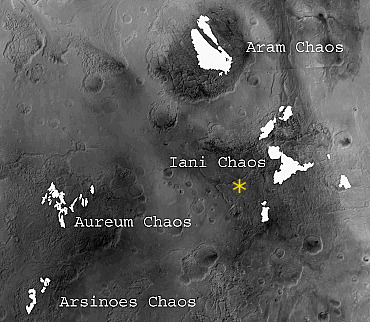
\includegraphics[width=0.45\linewidth]{sections/mars-solar-energy/mission-sites/images/iani-chaos-deposits.png}\\
  \caption[Map of light‐toned deposits in chaotic terrains in Margaritifer Terra]
          {Map of light‐toned deposits in chaotic terrains in Margaritifer Terra overlaid on a \ac{MOC} \ac{WA} mosaic. The mapped region covers \SI{9}{\degree}S – \SI{4}{\degree}N latitude and \SI{12}{\degree} – \SI{32}{\degree}W longitude. Taken from \citeother{Glotch2007}. The yellow asterisk indicates the \ac{HiRISE} \ac{DTM} location in Western Iani Chaos which was used for mission scenario simulation.}
  \label{fig:mission-site-iani-chaos}
\end{figure}

\refFig{fig:sub:western-iani-chaos-dtm} shows a section of the \ac{DTM} of Western Iani Chaos which was loaded on the rover's mission simulation plaform. The topography of the area is shown in \refFig{fig:sub:western-iani-chaos-dtm-altimetry}.

\vspace{0.5cm}

\begin{figure}[h]
\captionsetup[subfigure]{justification=centering}
%\vspace{-2ex}
	\centering
    %% setup sizes
    \setlength{\subfigureWidth}{0.50\textwidth}
    \setlength{\graphicsHeight}{90mm}
    %% kill hyper-link highlighting
    \hypersetup{hidelinks=true}%
    %% the figures
    \begin{subfigure}[t]{\subfigureWidth}
        \centering
        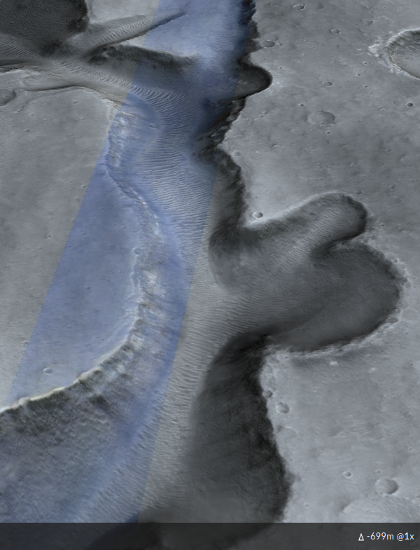
\includegraphics[height=\graphicsHeight]{sections/mars-solar-energy/mission-sites/images/western-iani-chaos-dtm.png}
        \subcaption{\ac{DTM}}
        \label{fig:sub:western-iani-chaos-dtm}
    \end{subfigure}\hfill
    \begin{subfigure}[t]{\subfigureWidth}
        \centering
        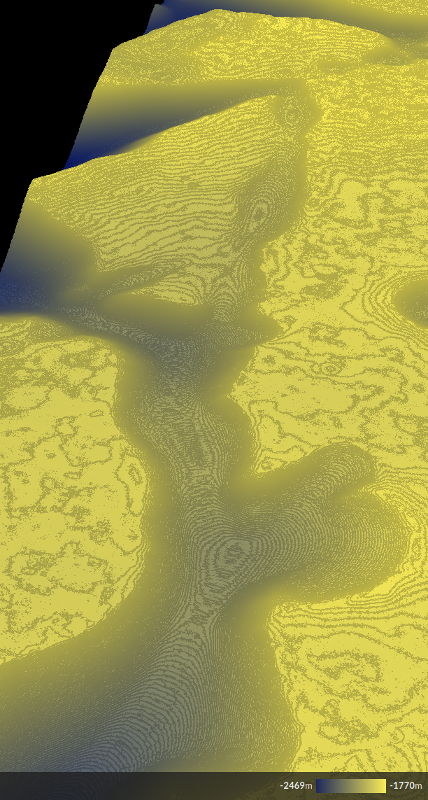
\includegraphics[height=\graphicsHeight]{sections/mars-solar-energy/mission-sites/images/western-iani-chaos-dtm-altimetry.png}
  		\subcaption{Topography}
		\label{fig:sub:western-iani-chaos-dtm-altimetry}
	\end{subfigure}\\[0.8ex]
    \caption[Western Iani Chaos HiRISE digital terrain model]
            {Western Iani Chaos \ac{HiRISE} \ac{DTM}. Taken from \citeother{AreoBrowser}. Image: \ac{NASA}/\ac{JPL}/University of Arizona.}
    \label{fig:western-iani-chaos}
\vspace{-2ex}
\end{figure}

\clearpage
\subsection{Ismenius Cavus}
\label{sec:MissionSites:IsmeniusCavus}
Ismenius Cavus is located at \SI{33.5}{\degree}N, \SI{17}{\degree}E, with elevations ranging from \SI{-3.5}{\kilo\meter} and \SI{-1.5}{\kilo\meter}. It is a basin where several fluvial valleys converge and is located ``at the junction between current mid-latitude ice deposits and low latitude clay minerals'', hosting science and resource regions of interest ``with both present ice and past lake sediments with clay minerals'' \citeother{Dehouck2010} \citeother{Dehouck2015}. Geologic context for this mission site area is provided with \refFig{fig:mission-site-ismenius-cavus}.

\begin{figure}[h]
  \centering
  \hypersetup{linkcolor=captionTextColor}
  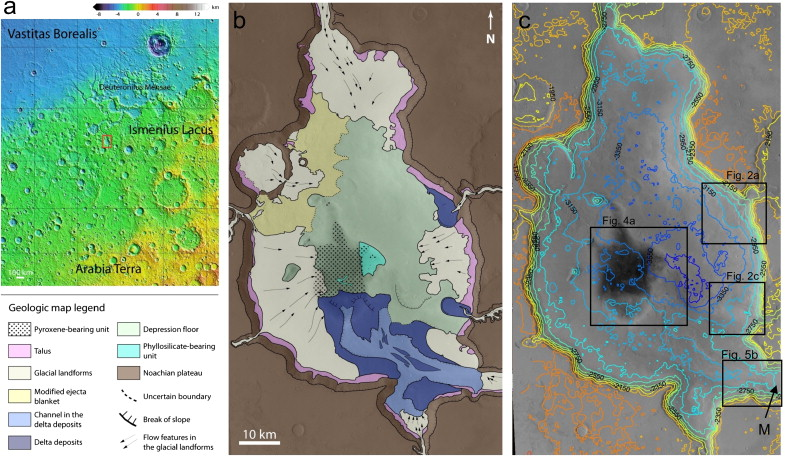
\includegraphics[width=0.6\linewidth]{sections/mars-solar-energy/mission-sites/images/ismenius-cavus.png}\\
  \caption[Geologic context of Ismenius Cavus mission site area]
          {Geologic context of Ismenius Cavus mission site area, taken from \citeother{Dehouck2010}. Location shown on a \ac{MOLA} reference map (a) and a geologic map of Ismenius Cavus (b). The yellow asterisk indicates the \ac{HiRISE} \ac{DTM} location which was used for mission scenario simulation.}
  \label{fig:mission-site-ismenius-cavus}
\end{figure}

% https://www.uahirise.org/dtm/dtm.php?ID=ESP_052945_2150

Supported science of interest are taken from \citeother{Dehouck2015}:
\begin{enumerate}[label=\textcolor{BulletBlue}{(\alph*)}]
    \item Potential for past habitability.
    \item Potential for organic matter with surface exposure.
    \item Noachian/Hesperian rocks with trapped atmospheric gases.
    \item High likelohood of surface-atmosphere exchange.
    \item Amazonian subsurface or high-latitude ice or sediment.
    \item Range of Martian geologic time; datable surfaces.
    \item Evidence of aqueous processes.
    \item Potential for interpreting relative ages.
    \item Near-surface ice, glacial or permafrost.
    \item Noachian or pre-Noachian bedrock units.
    \item Diversity of aeolian sediments and/or landforms.
\end{enumerate}

Supported resources of interest are also presented in \citeother{Dehouck2015} with clay minerals and water ice being two main resources for water. Furthermore, there is a potential for metal/silicon. These resources are located no more than \SI{3}{\meter} below the surface. Mobile material resources for construction purposes also exist.

\refFig{fig:sub:ismenius-cavus-dtm} shows a section of the \ac{DTM} which was loaded on the rover's mission simulation plaform. It features an exit breach in a well-preserved crater. The topography of the area is shown in \refFig{fig:sub:western-iani-chaos-dtm-altimetry}.
\vspace{0.5cm}

\begin{figure}[h]
\captionsetup[subfigure]{justification=centering}
\vspace{-2ex}
	\centering
    %% setup sizes
    \setlength{\subfigureWidth}{0.50\textwidth}
    \setlength{\graphicsHeight}{70mm}
    %% kill hyper-link highlighting
    \hypersetup{hidelinks=true}%
    %% the figures
    \begin{subfigure}[t]{\subfigureWidth}
        \centering
        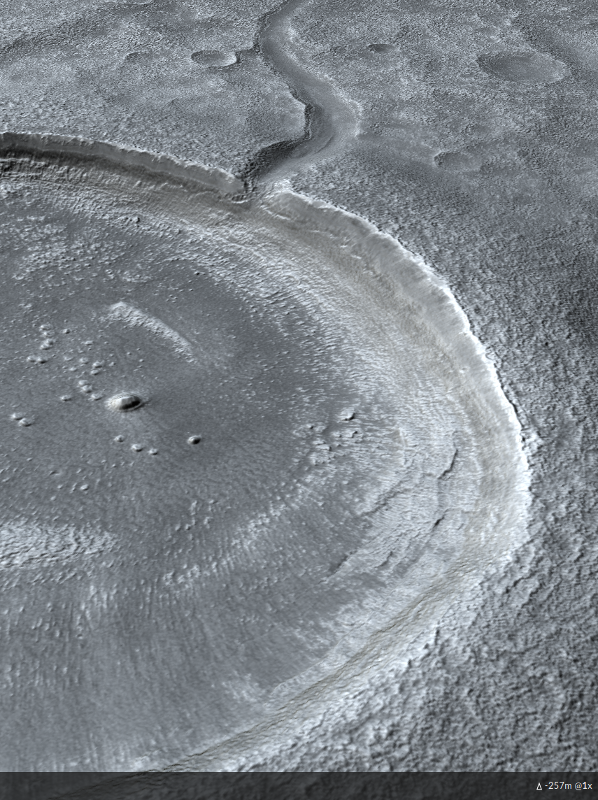
\includegraphics[height=\graphicsHeight]{sections/mars-solar-energy/mission-sites/images/ismenius-cavus-dtm.png}
        \subcaption{\ac{DTM}}
        \label{fig:sub:ismenius-cavus-dtm}
    \end{subfigure}\hfill
    \begin{subfigure}[t]{\subfigureWidth}
        \centering
        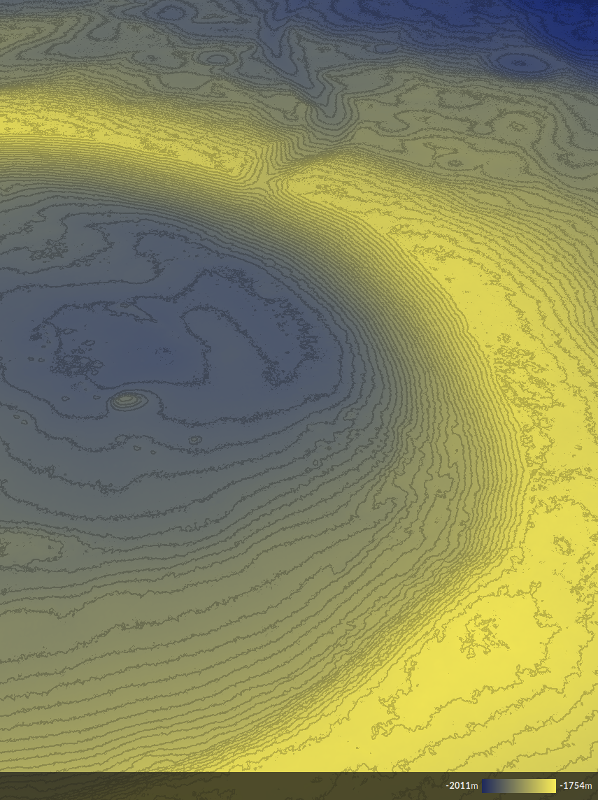
\includegraphics[height=\graphicsHeight]{sections/mars-solar-energy/mission-sites/images/ismenius-cavus-dtm-altimetry.png}
  		\subcaption{Topography}
		\label{fig:sub:ismenius-cavus-dtm-altimetry}
	\end{subfigure}\\[0.8ex]
    \caption[Ismenius Cavus HiRISE digital terrain model]
            {Ismenius Cavus \ac{HiRISE} \ac{DTM}, taken from \citeother{AreoBrowser}. Image: \ac{NASA}/\ac{JPL}/University of Arizona.}
    \label{fig:ismenius-cavus}
\vspace{-2ex}
\end{figure}

\subsection{Daily Insolation}
Worst and best case daily insolations presented in this section are considered when sizing the rover's \ac{SA}. Optical depth is typically around $\tau = 0.4$ on clear days \citemarsenv{Smith2019} and $1 \leq \tau \leq 1.5$ during local dust storms \citemarsenv{Lemmon2015}. Daily insolations $\tau > 1.5$ were only considered for global dust storm season ($\SI{180}{\degree} < L_{s} < \SI{360}{\degree}$). Year long daily insolations for $\tau = 0.4$ at both sites are shown in \refFig{fig:plot:solar-insolations-for-different-beta} where the selected $\beta$ inclination angles are combined with their optimal $\gamma_c$ orientation angles. Descriptions of these angles are found in Appendix \ref{sec:Appendix:OptimalAngles}.

\begin{figure}[h]
\captionsetup[subfigure]{justification=centering}
\vspace{-2ex}
\centering
    %% setup sizes
    \setlength{\subfigureWidth}{0.50\textwidth}
    \setlength{\graphicsHeight}{60mm}
    %% kill hyper-link highlighting
    \hypersetup{hidelinks=true}%
    %% the figures
    \begin{subfigure}[t]{\subfigureWidth}
        \centering
            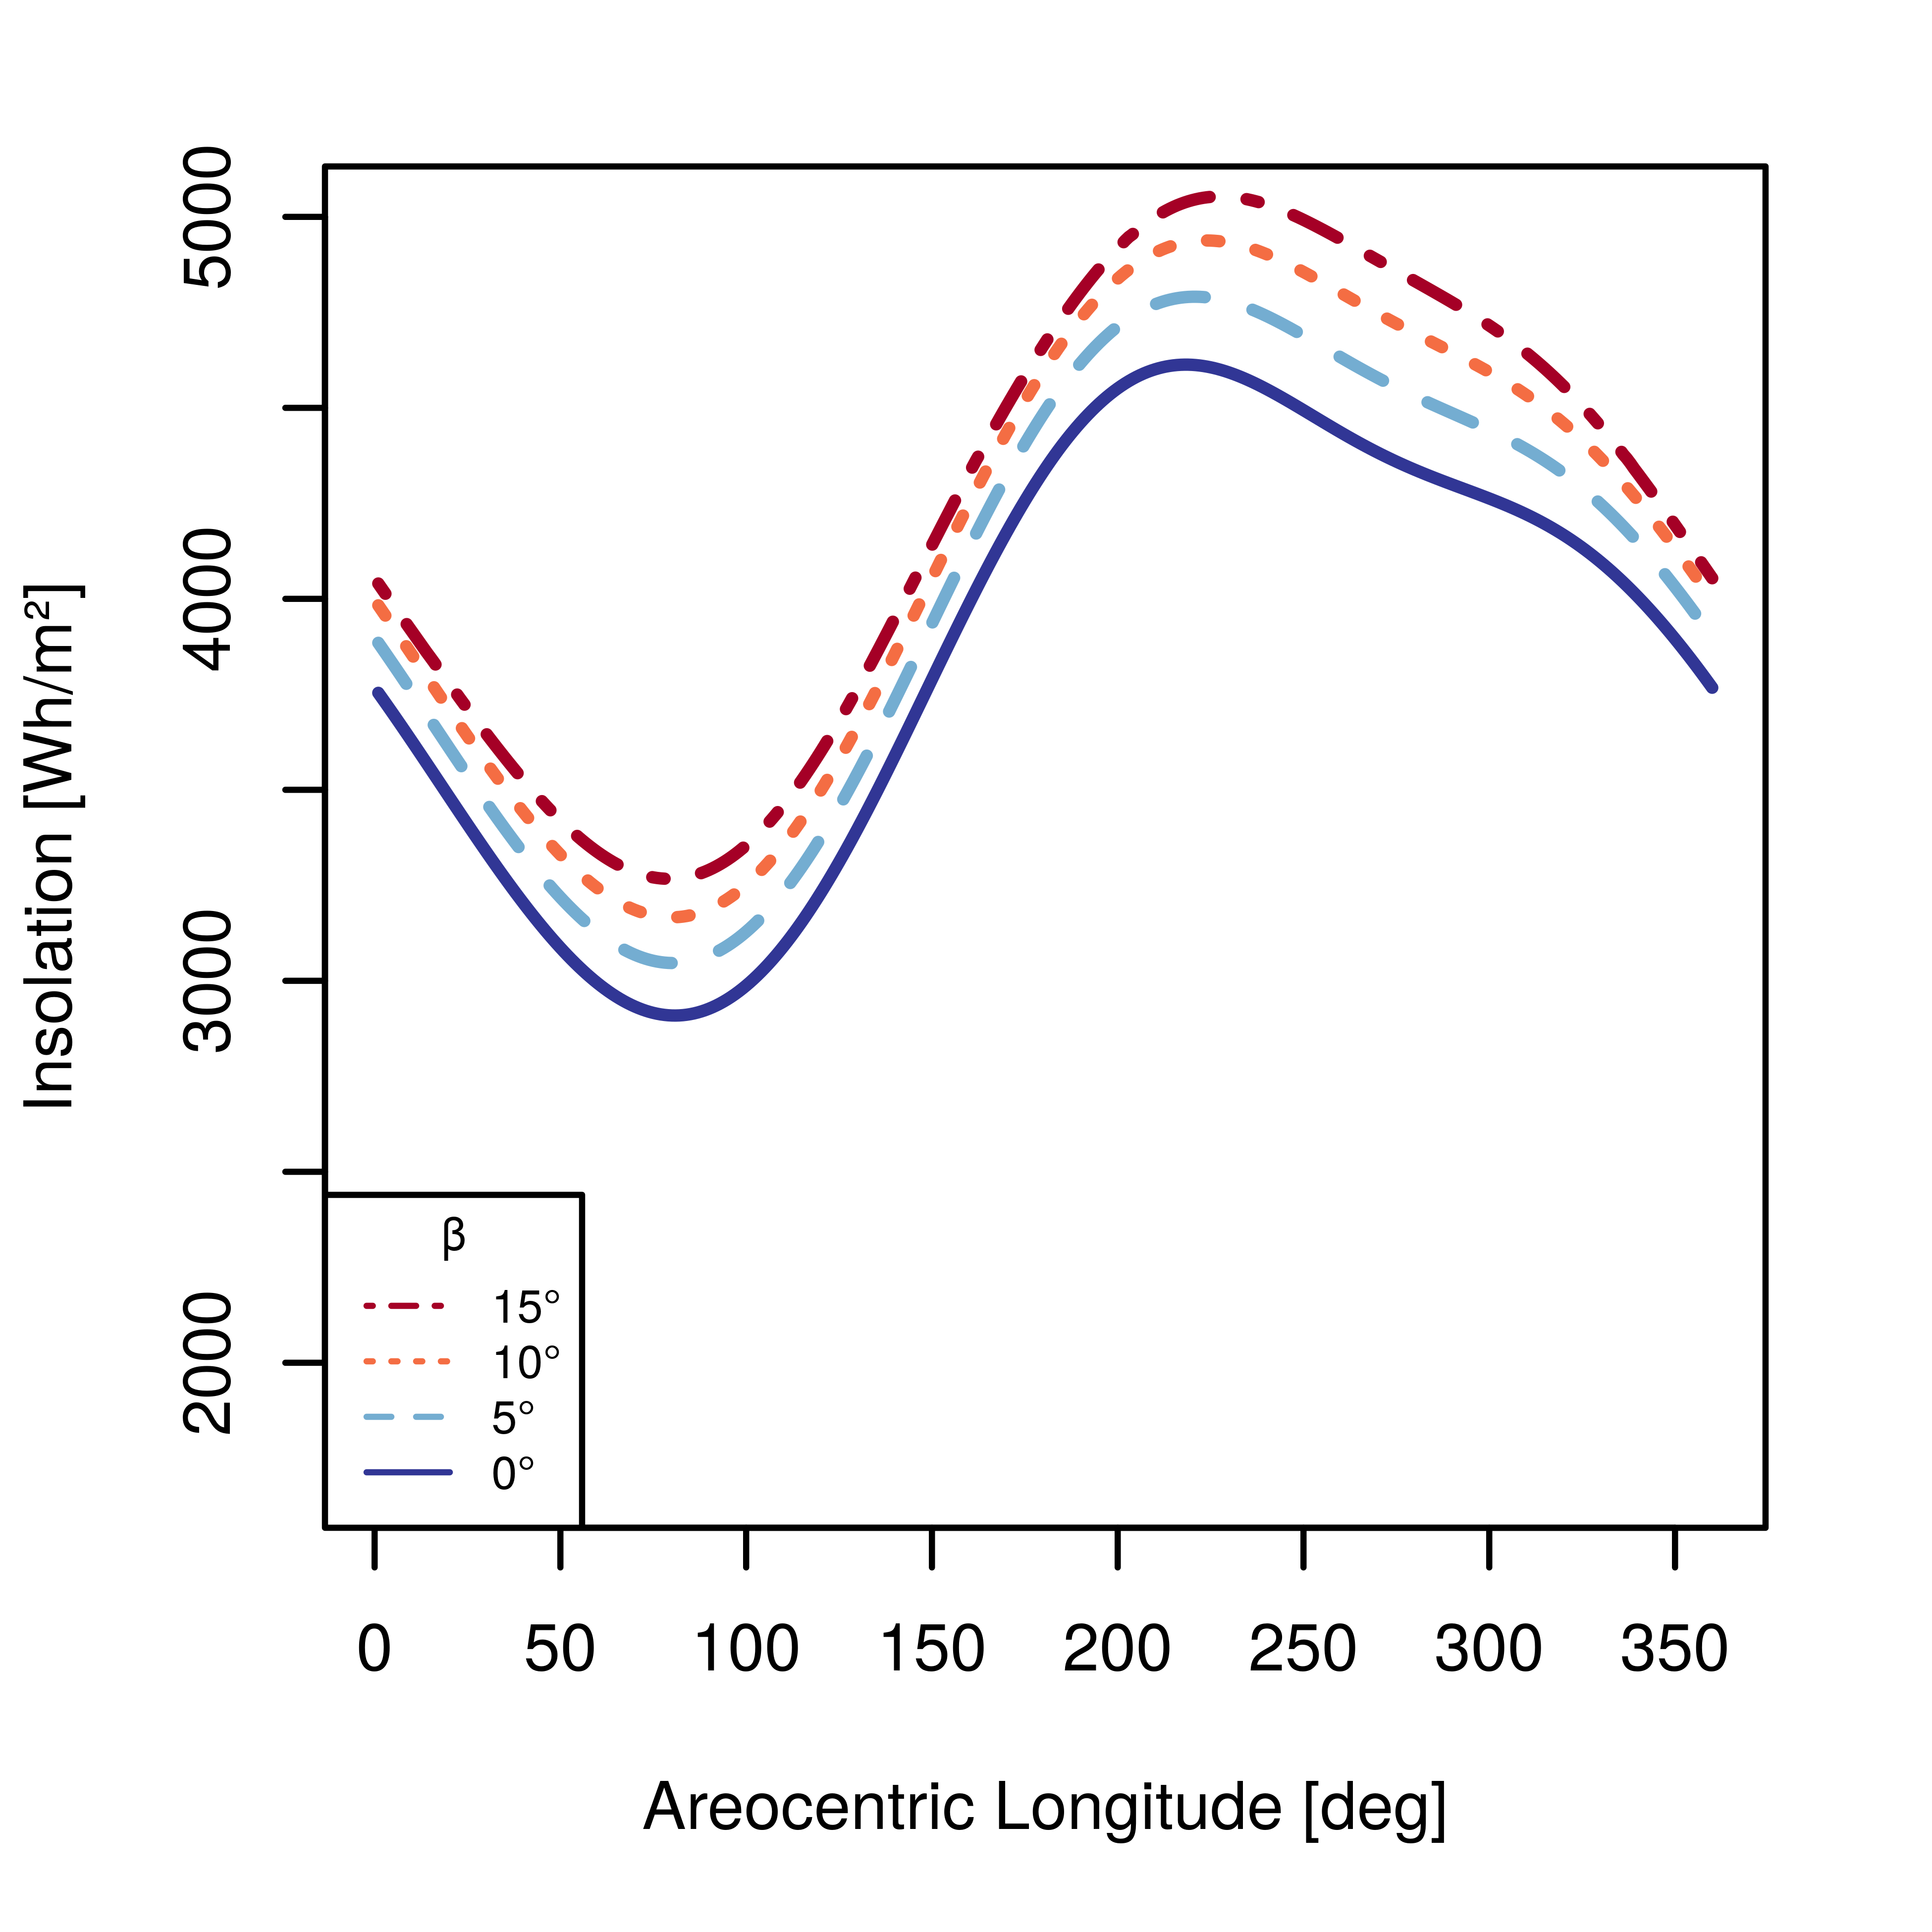
\includegraphics[height=\graphicsHeight]{sections/mars-solar-energy/mission-sites/plots/iani-chaos-solar-insolations-for-different-beta-inclinations.png}
            \subcaption{Iani Chaos.}
            \label{fig:plot:sub:solar-insolations-for-different-beta-iani-chaos}
    \end{subfigure}\hfill
    \begin{subfigure}[t]{\subfigureWidth}
        \centering
            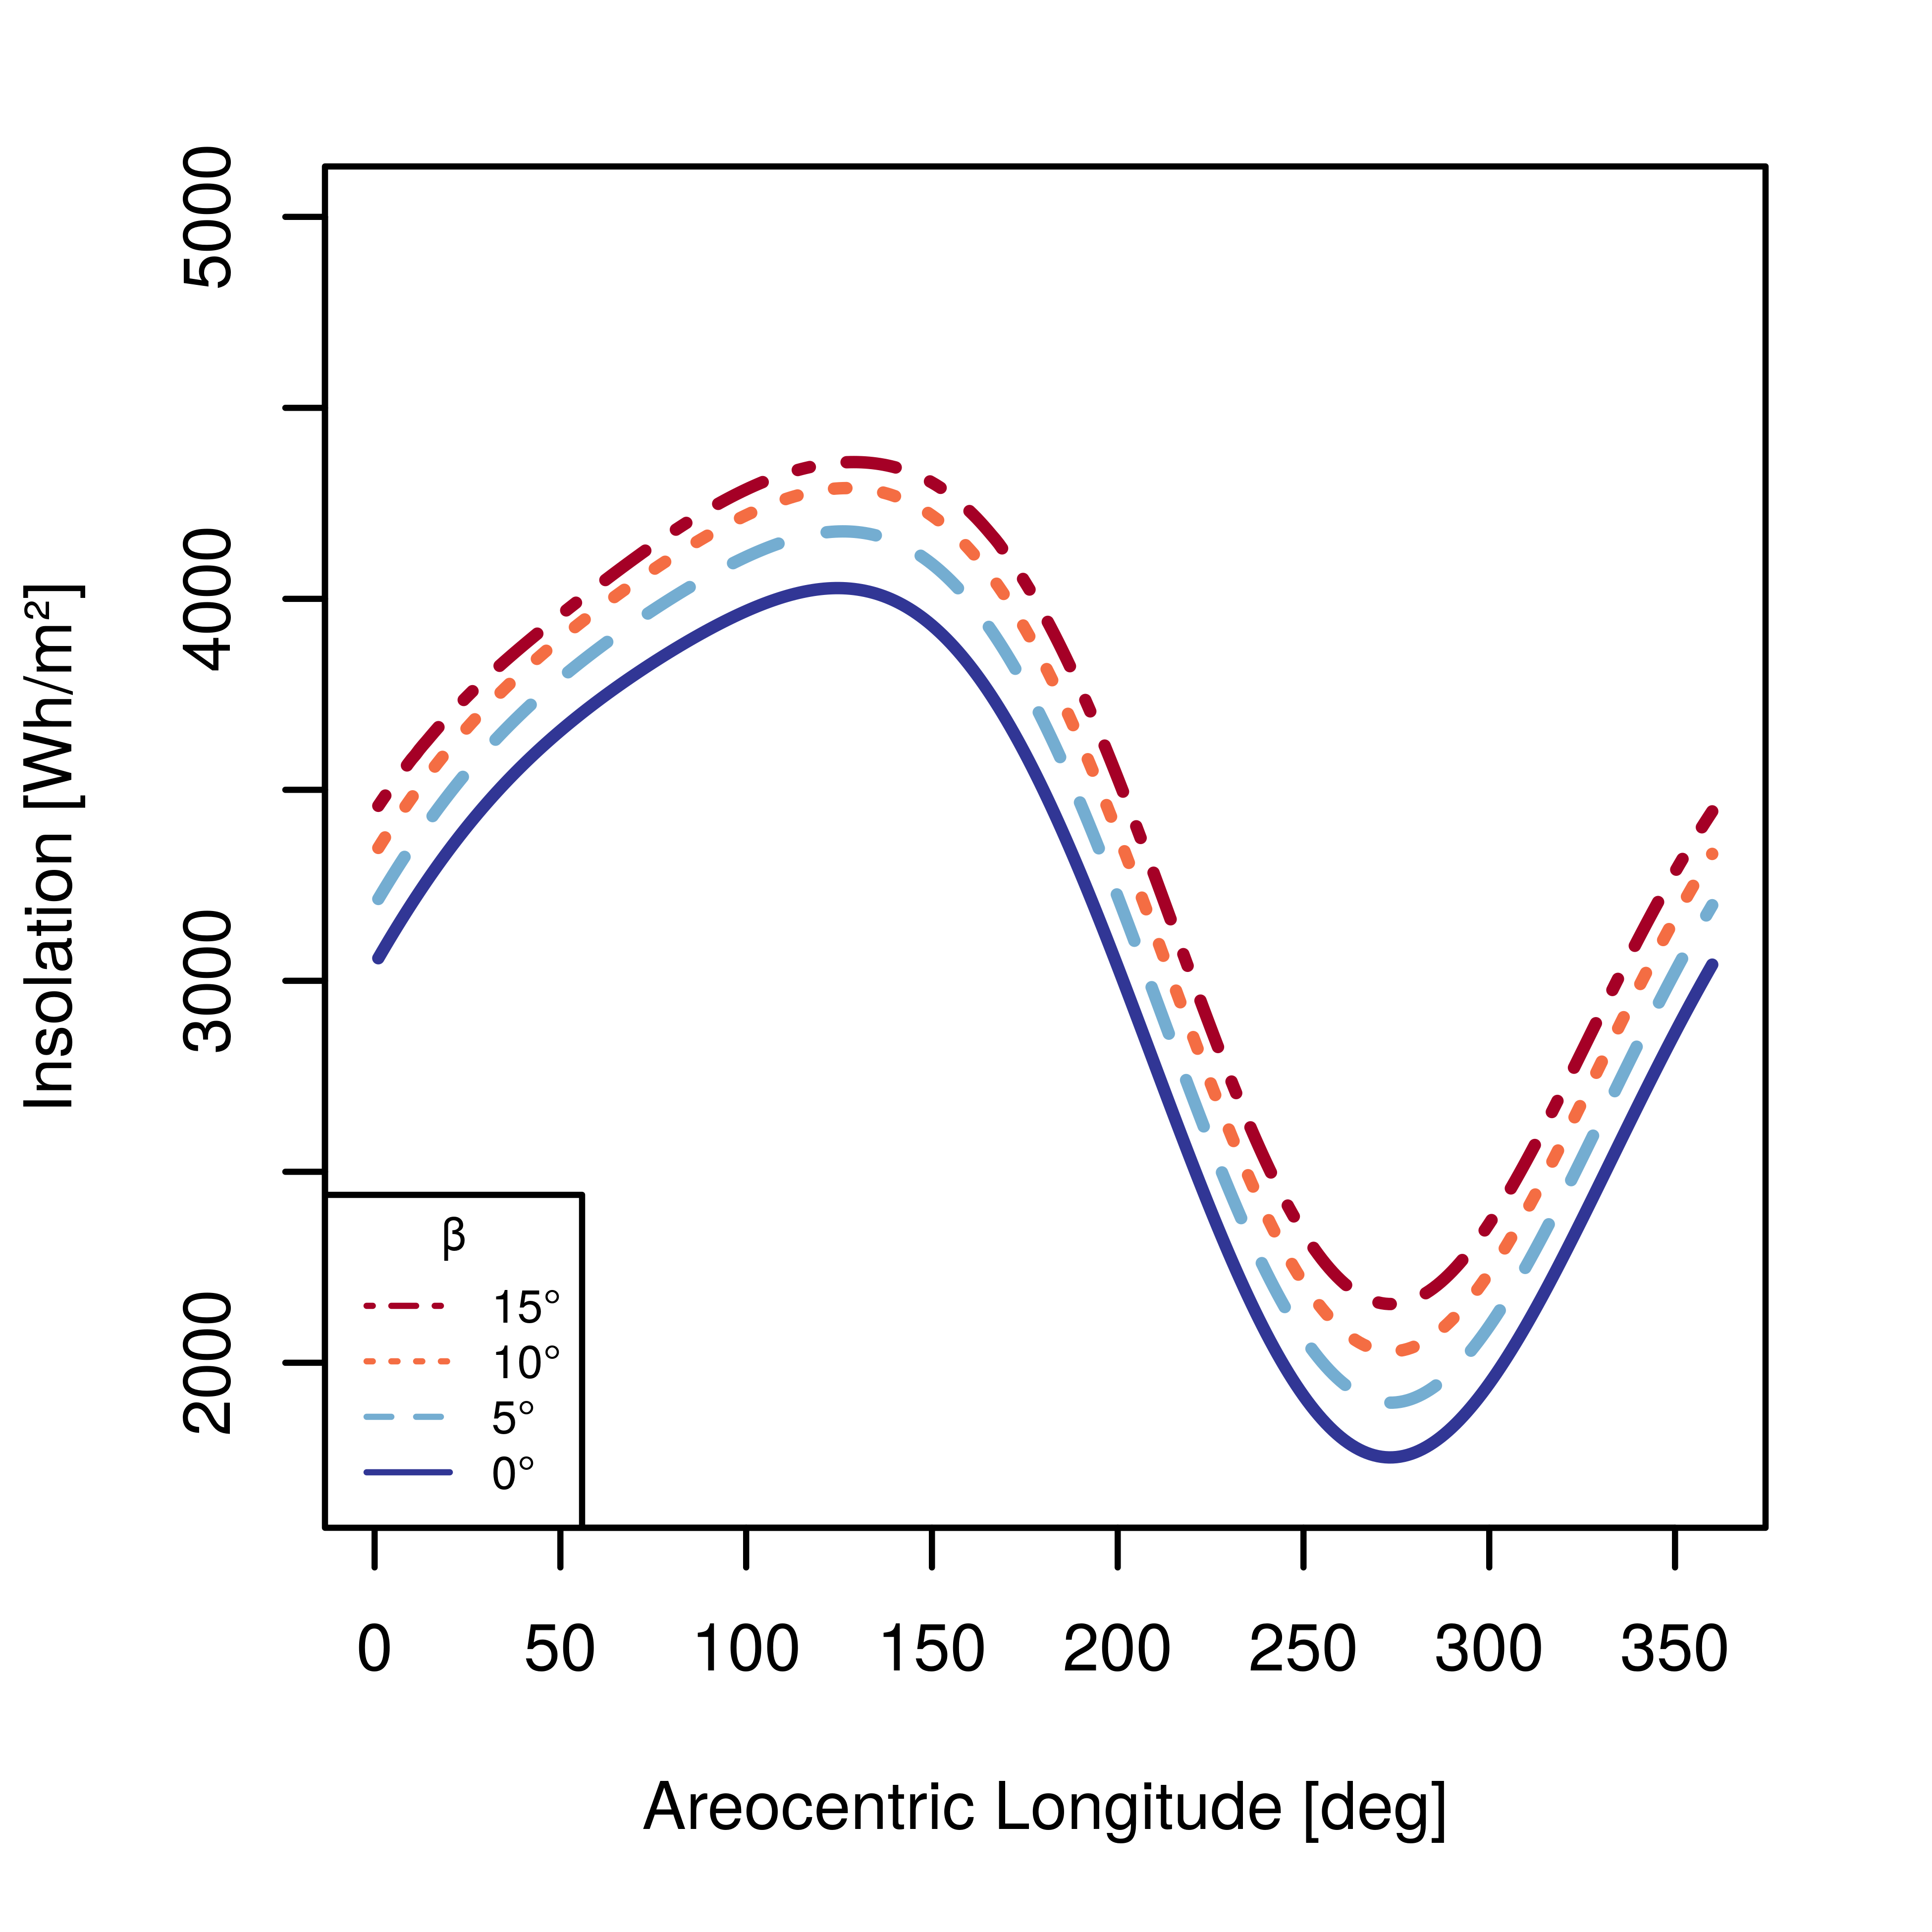
\includegraphics[height=\graphicsHeight]{sections/mars-solar-energy/mission-sites/plots/ismenius-cavus-solar-insolations-for-different-beta-inclinations.png}
            \subcaption{Ismenius Cavus.}
            \label{fig:plot:sub:solar-insolations-for-different-beta-ismenius-cavus}
    \end{subfigure}\\[0.8ex]
    \caption[Daily insolations at mission sites]
    {Daily insolations at mission sites for different combinations of surface inclination and orientation angles.}
    \label{fig:plot:solar-insolations-for-different-beta}
\vspace{-2ex}
\end{figure}

Large values of $\beta$ are typically preferred in terms of resulting insolation. However, constraints imposed on the rover's active suspension system imposes a limit on the attainable inclination. As such, the optimal $\beta$ angle from which maximum insolation can be achieved, henceforth referred to as $\beta_{opt}$, may not be attainable. In such cases, the best possible $\beta$ angle is targetted, hereinafter referred to as $\beta_{best}$. Body pitch commands of up to \SI{10}{\degree} are experimentally evaluated during steep slope climbing in \citeother{Cordes2018}. Modeling higher pitch angles resulted in poor wheel-ground contact angle, as shown in \refFig{fig:postures-sa-beta}. This is due to the wheel-steering axis having the same tilt as the rover's body. The rover's attainable tilt is thus restricted to a maximum of \SI{10}{\degree}.

\begin{figure}[h]
\captionsetup[subfigure]{justification=centering}
%\vspace{-2ex}
	\centering
    %% setup sizes
    \setlength{\subfigureWidth}{0.50\textwidth}
    \setlength{\graphicsHeight}{50mm}
    %% kill hyper-link highlighting
    \hypersetup{hidelinks=true}%
    %% the figures
    \begin{subfigure}[t]{\subfigureWidth}
        \centering
        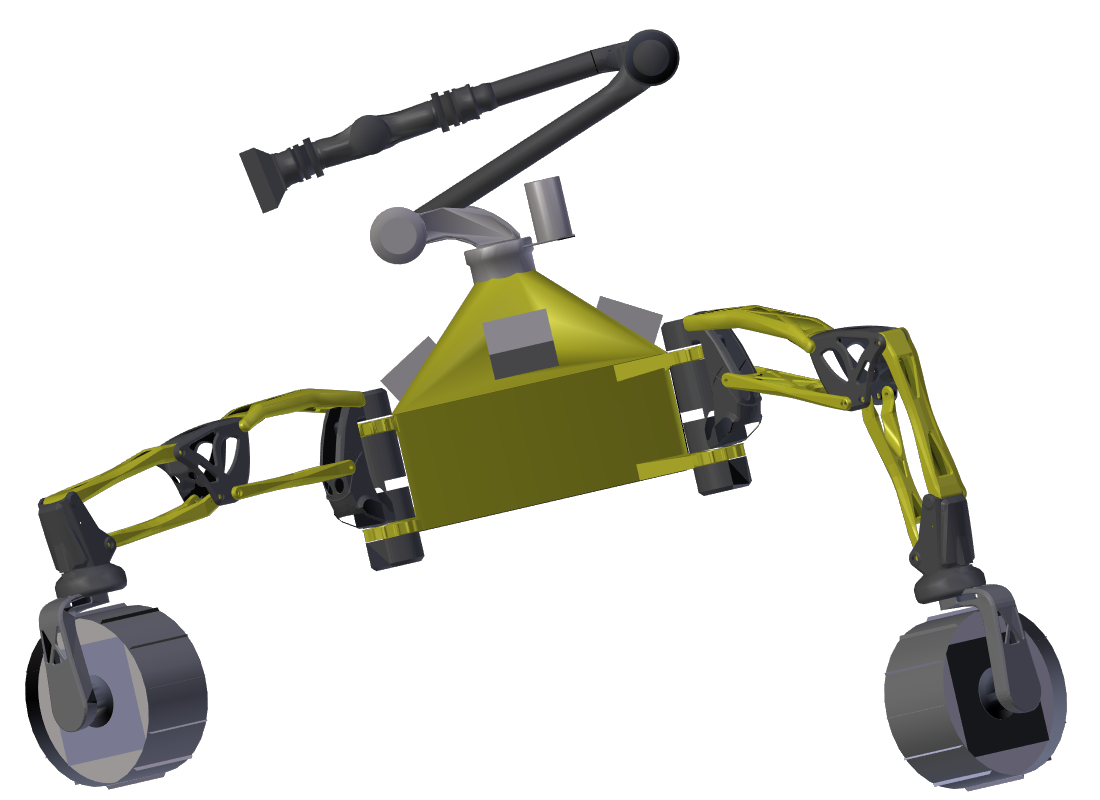
\includegraphics[height=\graphicsHeight]{sections/mars-solar-energy/mission-sites/images/sherpatt-render-surface-beta-13-deg.png}
        \subcaption{$\beta = \SI{13}{\degree}$}
        \label{fig:sub:postures-sa-beta-13-degree}
    \end{subfigure}\hfill
    \begin{subfigure}[t]{\subfigureWidth}
        \centering
        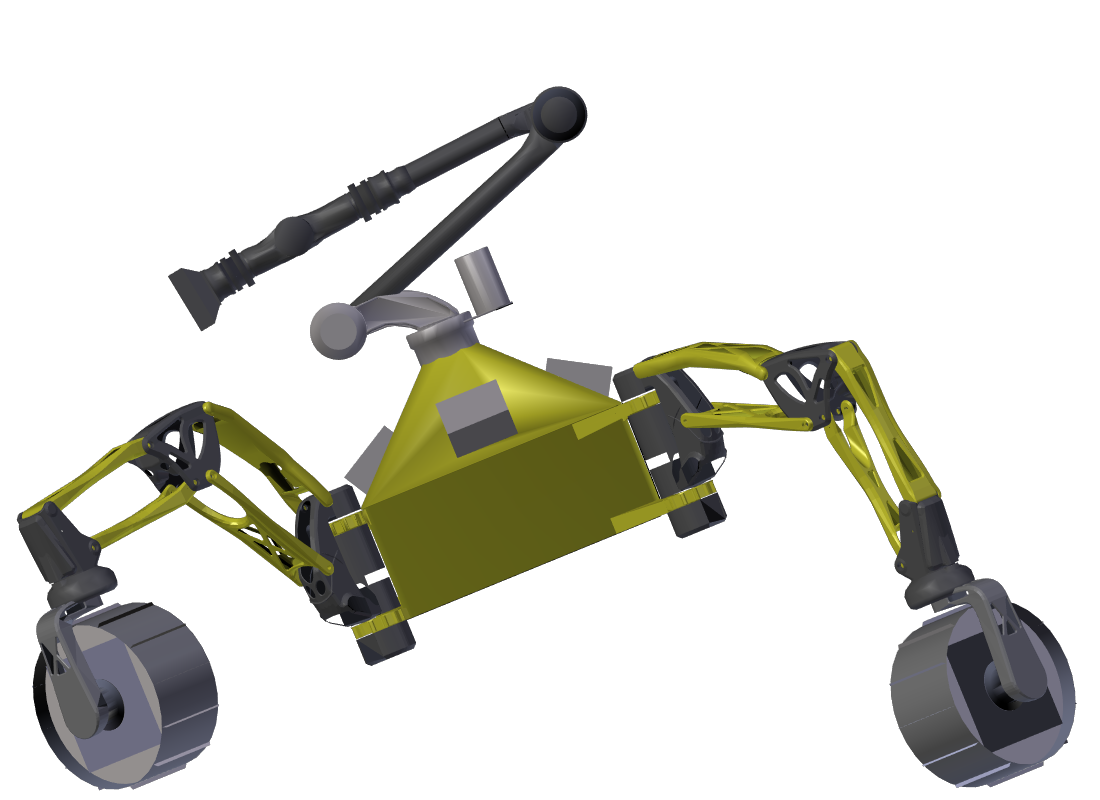
\includegraphics[height=\graphicsHeight]{sections/mars-solar-energy/mission-sites/images/sherpatt-render-surface-beta-22-deg.png}
  		\subcaption{$\beta = \SI{22}{\degree}$}
		\label{fig:sub:postures-sa-beta-22-degree}
	\end{subfigure}\\[0.8ex]
    \caption[SherpaTT body pitch \SI{13}{\degree} and \SI{22}{\degree}]
            {SherpaTT body pitch \SI{13}{\degree} and \SI{22}{\degree}.}
    \label{fig:postures-sa-beta}
\vspace{-2ex}
\end{figure}

\vspace{0.5cm}

Daily insolations on horizontal and inclined surfaces with $\beta_{best}=\pm\SI{10}{\degree}$\footnote{$\beta$ is positive in the northern hemisphere and negative in the southern hemisphere.} are presented in \refTab{tab:insolation-iani-chaos-clear-and-dusty-days} and \refTab{tab:insolation-iani-chaos-global-storm-days} for Iani Chaos and \refTab{tab:insolation-ismenius-cavus-clear-and-dusty-days} and \refTab{tab:insolation-ismenius-cavus-global-storm-days} for Ismenius Cavus. Gains obtained in daily insolation with an inclined surface are more pronounced for sites further away from the equator. For a typical optical depth of $\tau = 0.4$, the average daily insolation gain on the inclined surface is approximately \SI{7}{\percent} at Iani Chaos and \SI{9}{\percent} at Ismenius Cavus.
Due to the mostly diffuse composition of solar irradiance at higher optical depths, inclined surfaces become irrelevent during global dust storms. For $\tau \geq 2$, gains in daily insolation become negligeable at both mission sites.

\begin{table}[h]
\footnotesize
\centering
\caption[Worst- and best-case daily insolations for clear to dusty days at Iani Chaos]
{Worst- and best-case daily insolations for clear to dusty days at Iani Chaos. Daily insolation on an inclined surface $H_{\beta}$ was obtained with $\beta = \beta_{best} = \SI{-10}{\degree}$ and $\gamma_{c}$ set to optimal orientation angle.}
\label{tab:insolation-iani-chaos-clear-and-dusty-days}
\begin{tabular}{c|c|c|c|c|c|c|c|c|}
\cline{2-9}
\multicolumn{1}{l|}{} & \multicolumn{4}{c|}{\textbf{Worst Case}} & \multicolumn{4}{c|}{\textbf{Best Case}} \\ \hline
\multicolumn{1}{|c|}{$\tau$} & $L_{s}$ & $H_{h}$ & $H_{\beta}$ & $\%\:gain$ & $L_{s}$ & $H_{h}$ & $H_{\beta}$ & $\%\:gain$ \\ \hline
\multicolumn{1}{|c|}{\textbf{0.1}} & 80 & 3232 & 3721 & 15.13 & 221 & 5076 & 5695 & 12.19 \\ \hline
\multicolumn{1}{|c|}{\textbf{0.4}} & 81 & 2909 & 3166 & 8.85 & 218 & 4613 & 4933 & 6.93 \\ \hline
\multicolumn{1}{|c|}{\textbf{0.5}} & 81 & 2812 & 3025 & 7.58 & 218 & 4473 & 4736 & 5.89 \\ \hline
\multicolumn{1}{|c|}{\textbf{1.0}} & 82 & 2391 & 2479 & 3.67 & 214 & 3855 & 3959 & 2.69 \\ \hline
\multicolumn{1}{|c|}{\textbf{1.5}} & 82 & 2087 & 2125 & 1.81 & 213 & 3403 & 3444 & 1.19 \\ \hline
\end{tabular}
\end{table}


\vspace{0.5cm}

\begin{table}[h]
\footnotesize
\centering
\caption[Worst- and best-case daily insolations for global storm days at Iani Chaos]
{Worst- and best-case daily insolations for clear to global storm days at Iani Chaos. Daily insolation on an inclined surface $H_{\beta}$ was obtained with $\beta = \beta_{best} = \SI{-10}{\degree}$ and $\gamma_{c}$ set to optimal orientation angle.}
\label{tab:insolation-iani-chaos-global-storm-days}
\begin{tabular}{c|c|c|c|c|c|c|c|c|}
\cline{2-9}
\multicolumn{1}{l|}{} & \multicolumn{4}{c|}{\textbf{Worst Case}} & \multicolumn{4}{c|}{\textbf{Best Case}} \\ \hline
\multicolumn{1}{|c|}{$\tau$} & $L_{s}$ & $H_{h}$ & $H_{\beta}$ & $\%\:gain$ & $L_{s}$ & $H_{h}$ & $H_{\beta}$ & $\%\:gain$ \\ \hline
\multicolumn{1}{|c|}{\textbf{2.0}} & 360 & 2516 & 2519 & 0.10 & 212 & 3053 & 3066 & 0.42 \\ \hline
\multicolumn{1}{|c|}{\textbf{2.5}} & 360 & 2247 & 2243 & -0.18 & 211 & 2724 & 2723 & -0.02 \\ \hline
\multicolumn{1}{|c|}{\textbf{3.0}} & 360 & 1991 & 1985 & -0.32 & 210 & 2412 & 2406 & -0.27 \\ \hline
\multicolumn{1}{|c|}{\textbf{3.5}} & 360 & 1771 & 1763 & -0.45 & 210 & 2142 & 2134 & -0.37 \\ \hline
\multicolumn{1}{|c|}{\textbf{4.0}} & 360 & 1579 & 1572 & -0.44 & 209 & 1910 & 1901 & -0.47 \\ \hline
\multicolumn{1}{|c|}{\textbf{4.5}} & 360 & 1414 & 1406 & -0.54 & 209 & 1709 & 1700 & -0.54 \\ \hline
\multicolumn{1}{|c|}{\textbf{5.0}} & 360 & 1268 & 1261 & -0.58 & 209 & 1533 & 1523 & -0.62 \\ \hline
\end{tabular}
\end{table}


\vspace{0.5cm}

\begin{table}[h]
\footnotesize
\centering
\caption[Worst- and best-case daily insolations for clear to dusty days at Ismenius Cavus]
{Worst- and best-case daily insolations for clear to dusty days at Ismenius Cavus. Daily insolation on an inclined surface $H_{\beta}$ was obtained with $\beta = \beta_{best} = \SI{10}{\degree}$ and $\gamma_{c}$ set to optimal orientation angle.}
\label{tab:insolation-ismenius-cavus-clear-and-dusty-days}
\begin{tabular}{c|c|c|c|c|c|c|c|c|}
\cline{2-9}
\multicolumn{1}{l|}{} & \multicolumn{4}{c|}{\textbf{Worst Case}} & \multicolumn{4}{c|}{\textbf{Best Case}} \\ \hline
\multicolumn{1}{|c|}{$\tau$} & $L_{s}$ & $H_{h}$ & $H_{\beta}$ & $\%\:gain$ & $L_{s}$ & $H_{h}$ & $H_{\beta}$ & $\%\:gain$ \\ \hline
\multicolumn{1}{|c|}{\textbf{0.1}} & 274 & 2102 & 2762 & 31.42 & 127 & 4421 & 4925 & 11.40 \\ \hline
\multicolumn{1}{|c|}{\textbf{0.4}} & 273 & 1752 & 2030 & 15.85 & 125 & 4028 & 4289 & 6.49 \\ \hline
\multicolumn{1}{|c|}{\textbf{0.5}} & 273 & 1655 & 1869 & 12.93 & 124 & 3908 & 4122 & 5.48 \\ \hline
\multicolumn{1}{|c|}{\textbf{1.0}} & 273 & 1284 & 1345 & 4.75 & 121 & 3378 & 3461 & 2.44 \\ \hline
\multicolumn{1}{|c|}{\textbf{1.5}} & 273 & 1045 & 1061 & 1.57 & 120 & 2945 & 2973 & 0.96 \\ \hline
\end{tabular}
\end{table}


\vspace{0.5cm}

\begin{table}[h]
\footnotesize
\centering
\caption[Worst- and best-case daily insolations for global storm days at Ismenius Cavus]
{Worst- and best-case daily insolations for clear to global storm days at Ismenius Cavus. Daily insolation on an inclined surface $H_{\beta}$ was obtained with $\beta = \beta_{best} = \SI{10}{\degree}$ and $\gamma_{c}$ set to optimal orientation angle.}
\label{tab:insolation-ismenius-cavus-global-storm-days}
\begin{tabular}{c|c|c|c|c|c|c|c|c|}
\cline{2-9}
\multicolumn{1}{l|}{} & \multicolumn{4}{c|}{\textbf{Worst Case}} & \multicolumn{4}{c|}{\textbf{Best Case}} \\ \hline
\multicolumn{1}{|c|}{$\tau$} & $L_{s}$ & $H_{h}$ & $H_{\beta}$ & $\%\:gain$ & $L_{s}$ & $H_{h}$ & $H_{\beta}$ & $\%\:gain$ \\ \hline
\multicolumn{1}{|c|}{\textbf{2.0}} & 273 & 901 & 904 & 0.30 & 180 & 2155 & 2155 & 0.00 \\ \hline
\multicolumn{1}{|c|}{\textbf{2.5}} & 273 & 783 & 782 & -0.17 & 180 & 1899 & 1891 & -0.43 \\ \hline
\multicolumn{1}{|c|}{\textbf{3.0}} & 273 & 677 & 675 & -028 & 180 & 1664 & 1654 & -0.61 \\ \hline
\multicolumn{1}{|c|}{\textbf{3.5}} & 273 & 589 & 586 & -0.48 & 180 & 1467 & 1456 & -0.75 \\ \hline
\multicolumn{1}{|c|}{\textbf{4.0}} & 273 & 516 & 514 & -0.35 & 180 & 1300 & 1290 & -0.80 \\ \hline
\multicolumn{1}{|c|}{\textbf{4.5}} & 273 & 462 & 460 & -0.37 & 180 & 1158 & 1149 & -0.80 \\ \hline
\multicolumn{1}{|c|}{\textbf{5.0}} & 273 & 424 & 422 & -0.54 & 180 & 1038 & 1028 & -0.98 \\ \hline
\end{tabular}
\end{table}


The worst-case slope traverse is an on inclined surface facing opposite the equator. This can be mitigated by using the rover's suspension system to compensate with a tilt in the opposite direction, as illustrated in \refFig{fig:sub:rover-on-slope-beta} where $B$ denotes the slope surface inclination angle and $\beta$ the \ac{SA} surface inclination angle. This scenario will be further explored in \refSec{sec:Design:Simulation}. By way of example, at Ismenius Cavus for $\tau = 0.4$ and $L_{s}=\SI{270}{\degree}$, descending a \SI{30}{\degree} slope bearing North results in a daily insolation of \SI{319}{Whm^{-2}}. This can be increased to \SI{767}{Whm^{-2}} by decreasing $\beta$ from \SI{30}{\degree} to \SI{25}{\degree} after tilting the rover southwards by \SI{5}{\degree} so that $\beta < B$ with $\beta = \SI{25}{\degree}$. A \SI{10}{\degree} tilt would increase the daily insolation to \SI{1046}{Whm^{-2}} with $\beta = \SI{20}{\degree}$.


\begin{figure}[h]
\captionsetup[subfigure]{justification=centering}
%\vspace{-2ex}
	\centering
    %% setup sizes
    \setlength{\subfigureWidth}{0.50\textwidth}
    \setlength{\graphicsHeight}{40mm}
    %% kill hyper-link highlighting
    \hypersetup{hidelinks=true}%
    %% the figures
    \begin{subfigure}[t]{\subfigureWidth}
        \centering
        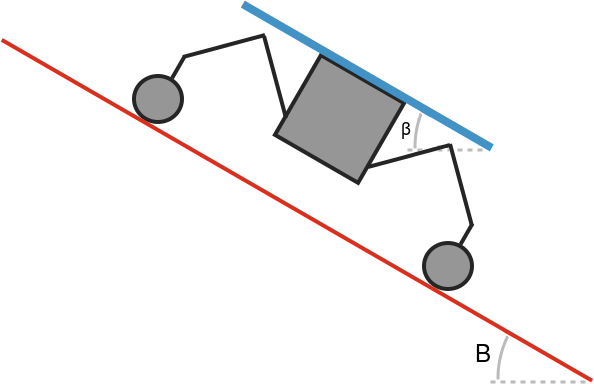
\includegraphics[height=\graphicsHeight]{sections/mars-solar-energy/mission-sites/images/stick-rover-beta-large.png}
        \subcaption{$\beta = B$}
        \label{fig:sub:rover-on-slope-beta-large}
    \end{subfigure}\hfill
    \begin{subfigure}[t]{\subfigureWidth}
        \centering
        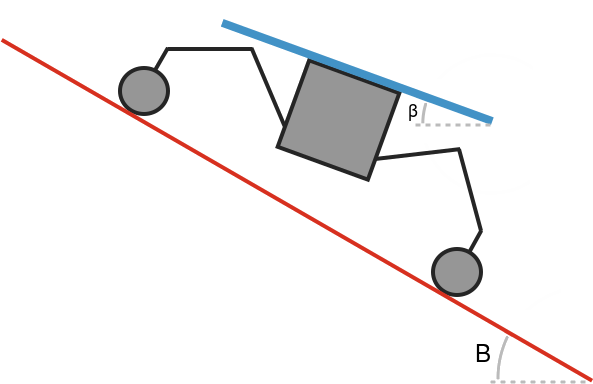
\includegraphics[height=\graphicsHeight]{sections/mars-solar-energy/mission-sites/images/stick-rover-beta-small.png}
  		\subcaption{$\beta < B$}
		\label{fig:sub:rover-on-slope-beta-small}
	\end{subfigure}\\[0.8ex]
    \caption[Slope compensation with active suspension system]
            {Slope compensation with active suspension system to reduce the \ac{SA} surface inclination angle. Slope inclination angle $B = \SI{30}{\degree}$. In (a), $\beta = B = \SI{30}{\degree}$. In (b), the rover is tilted  \SI{10}{\degree} in the opposite direction of the slope so that $\beta = \SI{20}{\degree}$.}
    \label{fig:sub:rover-on-slope-beta}
%\vspace{-2ex}
\end{figure}


\subsection{Summary}
Available solar insolation have been constrained by identifying two mission sites based on set of selection criteria. The need to navigate complex topographic morphologies at these sites also introduces considerations for \ac{SA} inclination strategies. Large differences in planetary latitudes between both sites ensures that several environmental variations are considered.
